\chapter{Cahier des charges}
\label{chap:3}

\noindent
Le but de ce mémoire consiste à développer un prototype capable de surveiller l'infrastructure de CERHIS et s'assurer du bon fonctionnement de celle-ci. De plus, ce système de monitoring doit pouvoir avertir un technicien lorsqu'un problème est détecté. Bien évidemment, pour accomplir cet objectif, le système devra acquérir des données sur le fonctionnement des différents dispositifs de CERHIS. Ces données devront être sauvegardées localement, mais aussi sur un serveur distant. Une interface web devra également être présente pour faciliter la visualisation de ces données, que cela soit dans le périmètre du centre hospitalier ou partout dans le monde. La figure \ref{fig:mon_archi_simple} reprend l'architecture simplifiée de ce système de monitoring.

~

\noindent
Pour simplifier la division du travail, la création du dispositif a été scindée en deux parties.
Une première partie majoritairement \textit{hardware} comportant le choix et l'assemblage de tous les composants nécessaires au développement du prototype. Cela englobe l'ordinateur requis pour tourner le logiciel, l'alimentation, la solution de communication et le logiciel qui permet aux différents composants de s'interfacer. Ensuite, une deuxième partie comprenant juste le logiciel nécessaire pour effectuer les tâches de monitoring. Cela comprend les fonctionnalités requises pour l'acquisition, traitement, stockage et visualisation des données. La présentation des spécificités de chaque partie se fera dans les sections suivantes (sections \ref{sec:cahier_proto} et \ref{sec:cahier_soft}).



\begin{figure}[ht!]
  \centering
  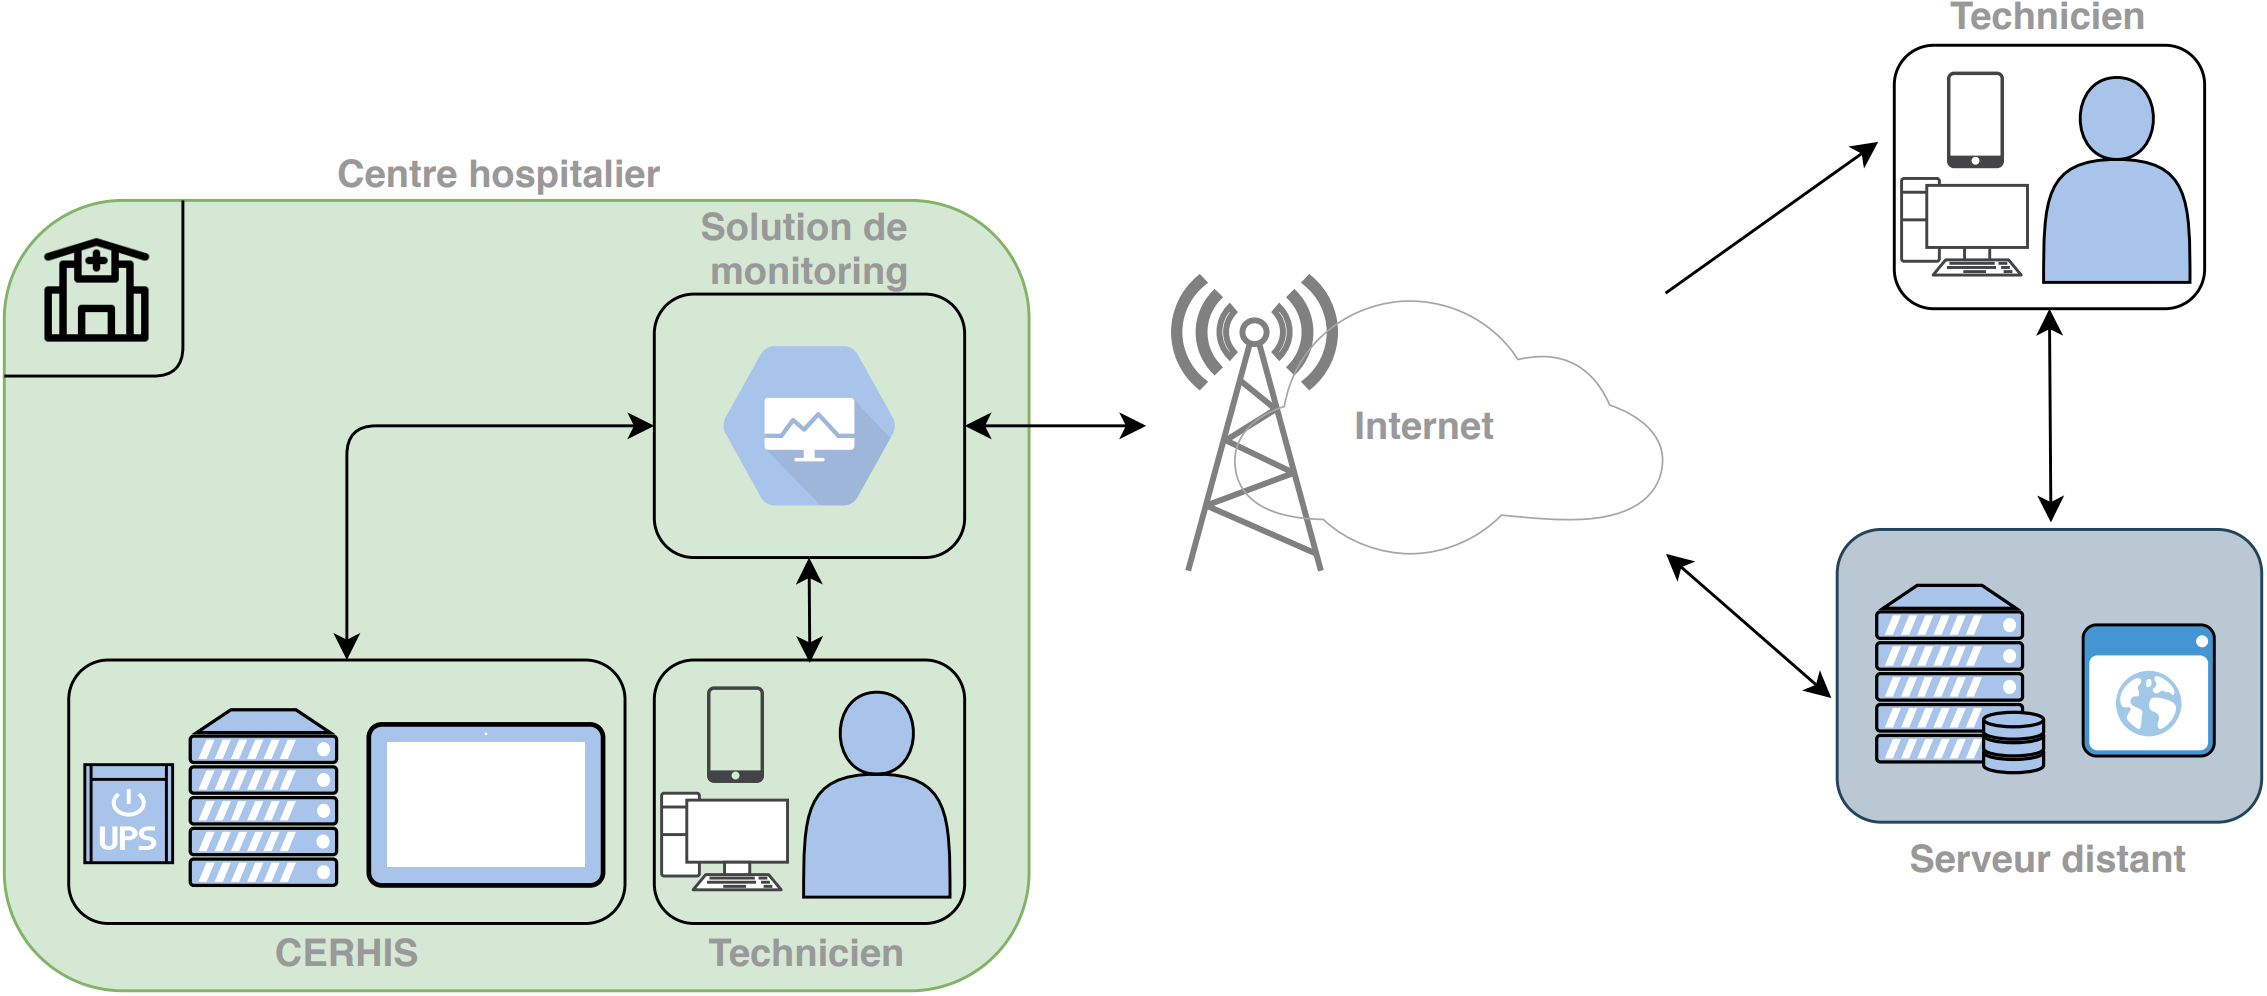
\includegraphics[width=\textwidth]{img/cahier_des_charges/baseline_archi.png}
  \caption{Architecture simplifiée de la solution de monitoring}
  \label{fig:mon_archi_simple}
\end{figure}

\section{Caractéristiques matérielles du dispositif}
\label{sec:cahier_proto}

Étant donné que le dispositif de monitoring sera utilisé dans des centres hospitaliers en Afrique centrale, il doit être capable de résister à certaines caractéristiques propres du milieu telles que la température. Voici la liste exhaustive de toutes les caractéristiques matérielles que le produit doit posséder :

~


\begin{itemize}
  \item Le prototype doit être robuste. Mes composants électroniques doivent notamment être capables de supporter des températures ambiantes supérieures à \SI{30}{\celsius} pendant de longues périodes. \cite{temperature_kinshasa}

  \item Le dispositif doit être capable de communiquer à distance, même lorsqu'une connexion à internet filaire n'est pas disponible. De ce fait, le prototype doit être capable de tirer parti d'une des technologies présentées dans la section 2 pour pouvoir envoyer des informations et des alertes.

  \item Le dispositif doit être d'apparence discrète, évitant d'attirer l'attention sur sa valeur.

  \item Le coût doit rester abordable et réaliste.

  \item Le dispositif doit posséder un système d'alimentation mixte capable d'alimenter le prototype pendant un ou deux jours en cas de passe du service électrique.

  \item Le boîtier doit être fermé hermétiquement pour empêcher des insectes d'y faire son nid.
\end{itemize}



\section{Fonctionnalités à implémenter}
\label{sec:cahier_soft}

Pour la section logiciel du dispositif, les fonctionnalités à implémenter peuvent encore être divisées en deux sous-sections : la solution de monitoring tournant sur le site, et le serveur distant capable de recevoir, stocker et afficher des données. Les fonctionnalités présentées ci-dessous seront alors divisées en suivant ces deux sous-sections.

~

\begin{itemize}
  \item \textbf{Solution de monitoring dans le centre hospitalier}
  \begin{itemize}
    \item Effectuer un mappage du réseau local de façon à trouver tous les appareils qui y sont connectés.

    \item Monitorer la présence des appareils connectés au réseau local. Si un appareil se déconnecte du réseau, pouvoir indiquer combien de temps est passé depuis sa dernière connexion.

    \item Monitorer l'état de fonctionnement du serveur de CERHIS.

    \item Envoi d'alertes par SMS.

    \item Envoi de données vers un serveur distant.

    \item Interface utilisateur permettant de facilement visualiser toutes les données.

    \item Vérifier le niveau de la batterie de CERHIS et l'état de charge des tablettes.

    \item Créer un historique de connexion des tablettes au serveur de CERHIS
  \end{itemize}

~

  \item \textbf{Serveur distant}
  \begin{itemize}
    \item Serveur capable de stocker les données envoyées depuis plusieurs centres hospitaliers.

    \item Interface utilisateur permettant de facilement visualiser toutes les données disponibles sur le serveur distant.
  \end{itemize}
\end{itemize}



\section{Priorité des tâches et méthodologie de travail}

\noindent
Les listes des fonctionnalités et caractéristiques présentes ci-dessus reprennent tout ce qui serait nécessaire pour avoir un produit fini. L'objectif de ce mémoire est bien évidemment d'essayer d'implémenter le maximum de fonctionnalités possibles. Cependant, le temps est limité et des imprévus peuvent survenir au long du chemin. De ce fait, les diverses fonctionnalités ont été classées par ordre de priorité afin de garantir que le prototype rendu à la fin de ce mémoire possède au moins un certain nombre de fonctionnalités.

~

\noindent
En premier lieu, c'était la sélection du matériel requis pour implémenter les fonctionnalités. Cela reprend, le choix de la plateforme, l'alimentation et la solution de communication. Cette tâche reprend aussi des tests sur la plateforme du projet de l'année précédente afin de vérifier si des changements étaient nécessaires.

~

\noindent
Deuxièmement, c'était l'implémentation de tout le code nécessaire pour lier les divers composants hardware. En particulier, l'implémentation du code essentiel pour mettre en marche la solution de communication. Ici s'ajoutent aussi les premiers essais afin de prouver le bon fonctionnement de la plateforme.

~

\noindent
Une fois la plateforme préliminaire choisie et testée, la possibilité de commencer à développer les différentes fonctionnalités du logiciel s'est ouverte. À nouveau, en raison du grand nombre de fonctionnalités requises, les plus cruciales ont été sélectionnées lors de réunions avec les parties prenantes. La liste ci-dessous présente les fonctionnalités triées par ordre décroissant de priorité :

~


\begin{itemize}
  \item Monitorer l'état du serveur, en particulier surveiller l'uptime de celui-ci et avertir un technicien en cas de modification anormale de la valeur.
  \item Mapper le réseau local.
  \item Surveiller la présence des dispositifs de CERHIS.
  \item Monitorer l'état de certains processus dans le serveur.
  \item Envoi des données vers un serveur distant.
  \item Interface web pour la visualisation des données
\end{itemize}

~

\noindent
Finalement, les dernières tâches reprennent la finalisation d'un boîtier permettant de loger les différents composants électroniques et des tests approfondis pour s'assurer du bon fonctionnement et la fiabilité de la solution de monitoring.

~

\noindent
Pour essayer d'être le plus efficace possible, la méthodologie de travail consistait à écrire toutes les tâches liées à ce projet sur des notes Post-it. Les Post-its orange représentaient les missions liées au software, et les jaunes correspondaient aux missions liées au hardware. Chaque note possédait aussi un numéro coïncidant avec la priorité de la tâche. Le critère de sélection était en premier lieu la couleur, orange prioritaire sur le jaune, et ensuite la priorité (lorsque les Post-its avaient tous la même couleur).
